\section{Signal discrimination}\label{sec:sigdiscr}
The production cross section for the signal processes \tHq, \tHW, and \ttH\ is only a few fb (even with inverted couplings, $\Ct=-1$), resulting in a small signal to background ratio even for a tight selection.
A multivariate method is hence employed to train a discriminator to separate \tHq\ signal events from background.
Several methods have been studied, with the best performance obtained from a gradient boosted decision tree (BDT) classifier using a maximum tree depth of three and an ensemble of 800 trees.
Two BDTs are trained separately for the same-sign dilepton and the three lepton channel on simulated events to separate the \tHq\ process either from an admixture of \ttW\ and \ttZ\ (in short \ttV), or from \ttbar.
Events from \tHW\ and \ttH\ production, while counted as signal events in the interpretation, share the kinematic characteristics of \ttV\ events and are not used in the classifier training.

Three broad categories of discriminating observables are used: related to forward jet activity; related to jet and \cPqb-jet multiplicities; and related to kinematic properties of leptons as well as their total charge.
Table~\ref{tab:bdtinputs} lists the 10 input variables used in the final discriminants.
Many combinations of kinematic variables were constructed to perform the discrimination between signal and background with the chosen set of variables giving the best performance in the separation.
The same or equivalent input variables are found to perform well both for three lepton and same-sign dilepton channels and both for training against \ttV\ and against \ttbar.

\begin{table}[h!]
\centering
\begin{tabular}{lp{12cm}}
 \hline
% & \textbf{Description}\\
& Number of jets with $\pt>25\GeV$, $|\eta|<2.4$\\
& Maximum $|\eta|$ of any (non-\cPqb-tagged) jet (``forward jet'')\\
& Sum of lepton charges \\
& Number of non-\cPqb-tagged jets with $|\eta|>1.0$\\
& $\Delta \eta$ between forward light jet and leading \cPqb-tagged jet\\
& $\Delta \eta$ between forward light jet and sub-leading \cPqb-tagged jet \\ %(set to -1 in events with only one tagged jet) \\
& $\Delta \eta$ between forward light jet and closest lepton\\
& $\Delta \phi$ of same-sign lepton pair\\
& Minimum $\Delta R$ between any two leptons\\
& \pt\ of sub-leading (or $3^{rd}$) lepton\\ \hline
\end{tabular}
\caption{Input variables to the signal discrimination classifier.}
\label{tab:bdtinputs}
\end{table}

The distributions for some of the BDT input variables are shown in Figures~\ref{fig:2lss_inputs_mm},~\ref{fig:2lss_inputs_em} and~\ref{fig:dist_likelihoodselection_PDFs_3l}, comparing observed data and predicted yields.
The analysis has been developed while blinded to the distributions of the
observed events passing the signal selection.

\begin{figure}[!htb]
  \centering
    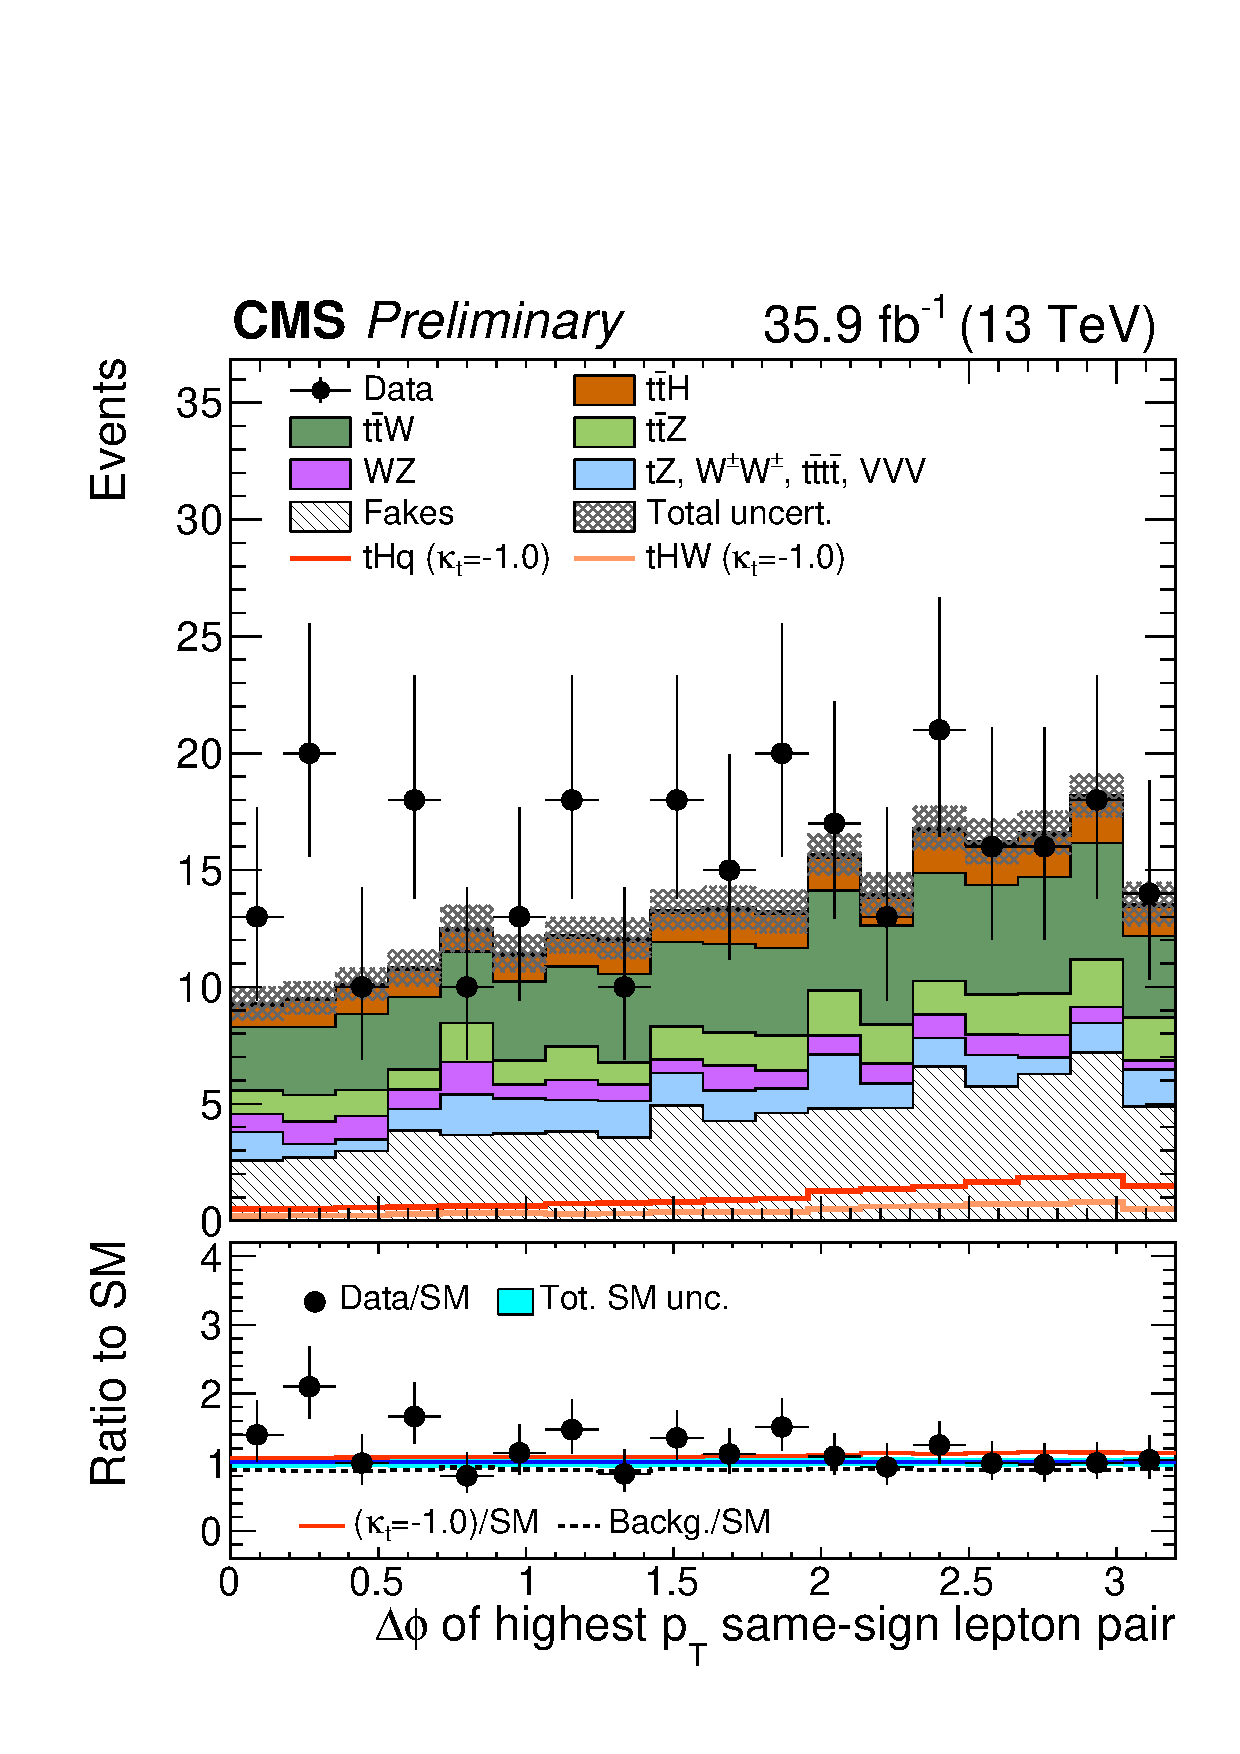
\includegraphics[width=0.32\linewidth]{Figures/polished/dPhiHighestPtSSPair_mm.pdf}
    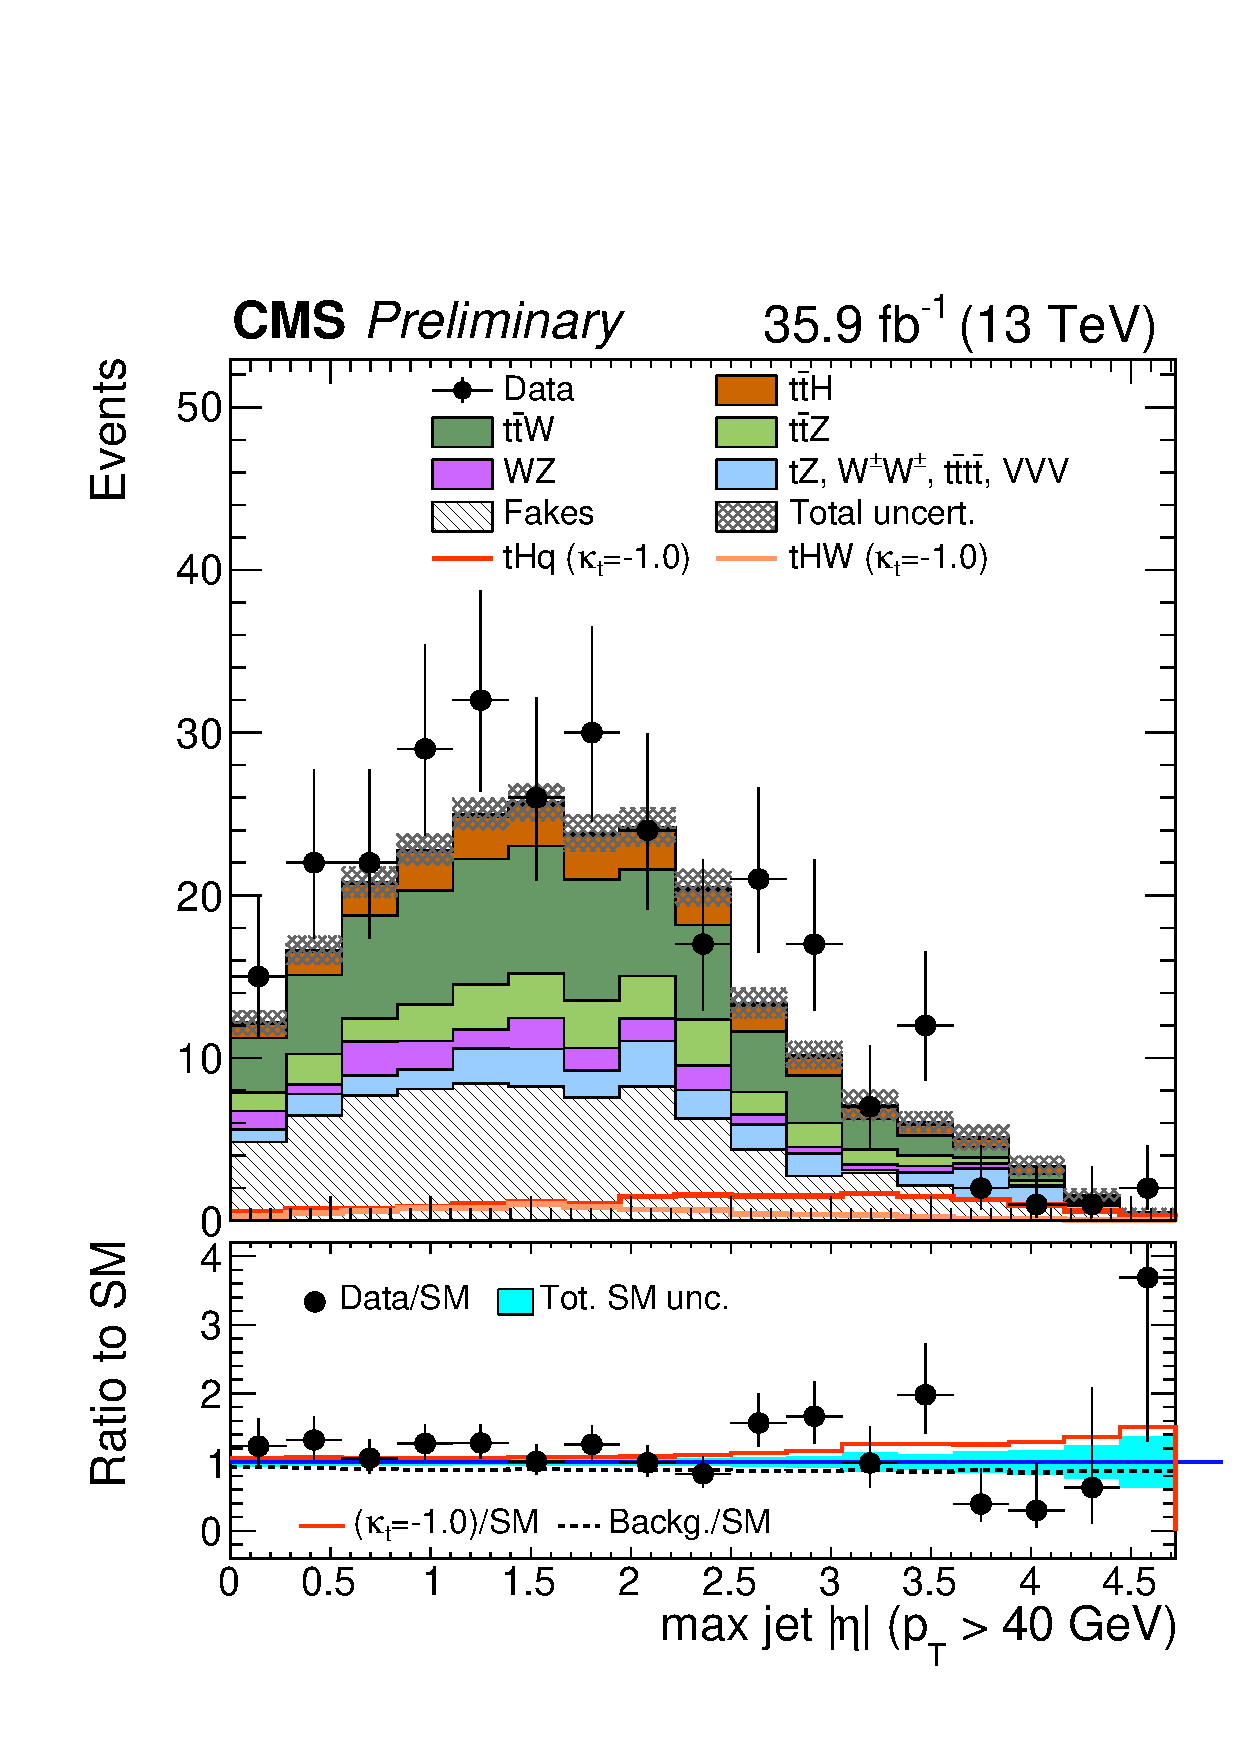
\includegraphics[width=0.32\linewidth]{Figures/polished/maxEtaJet25_40_mm.pdf}
    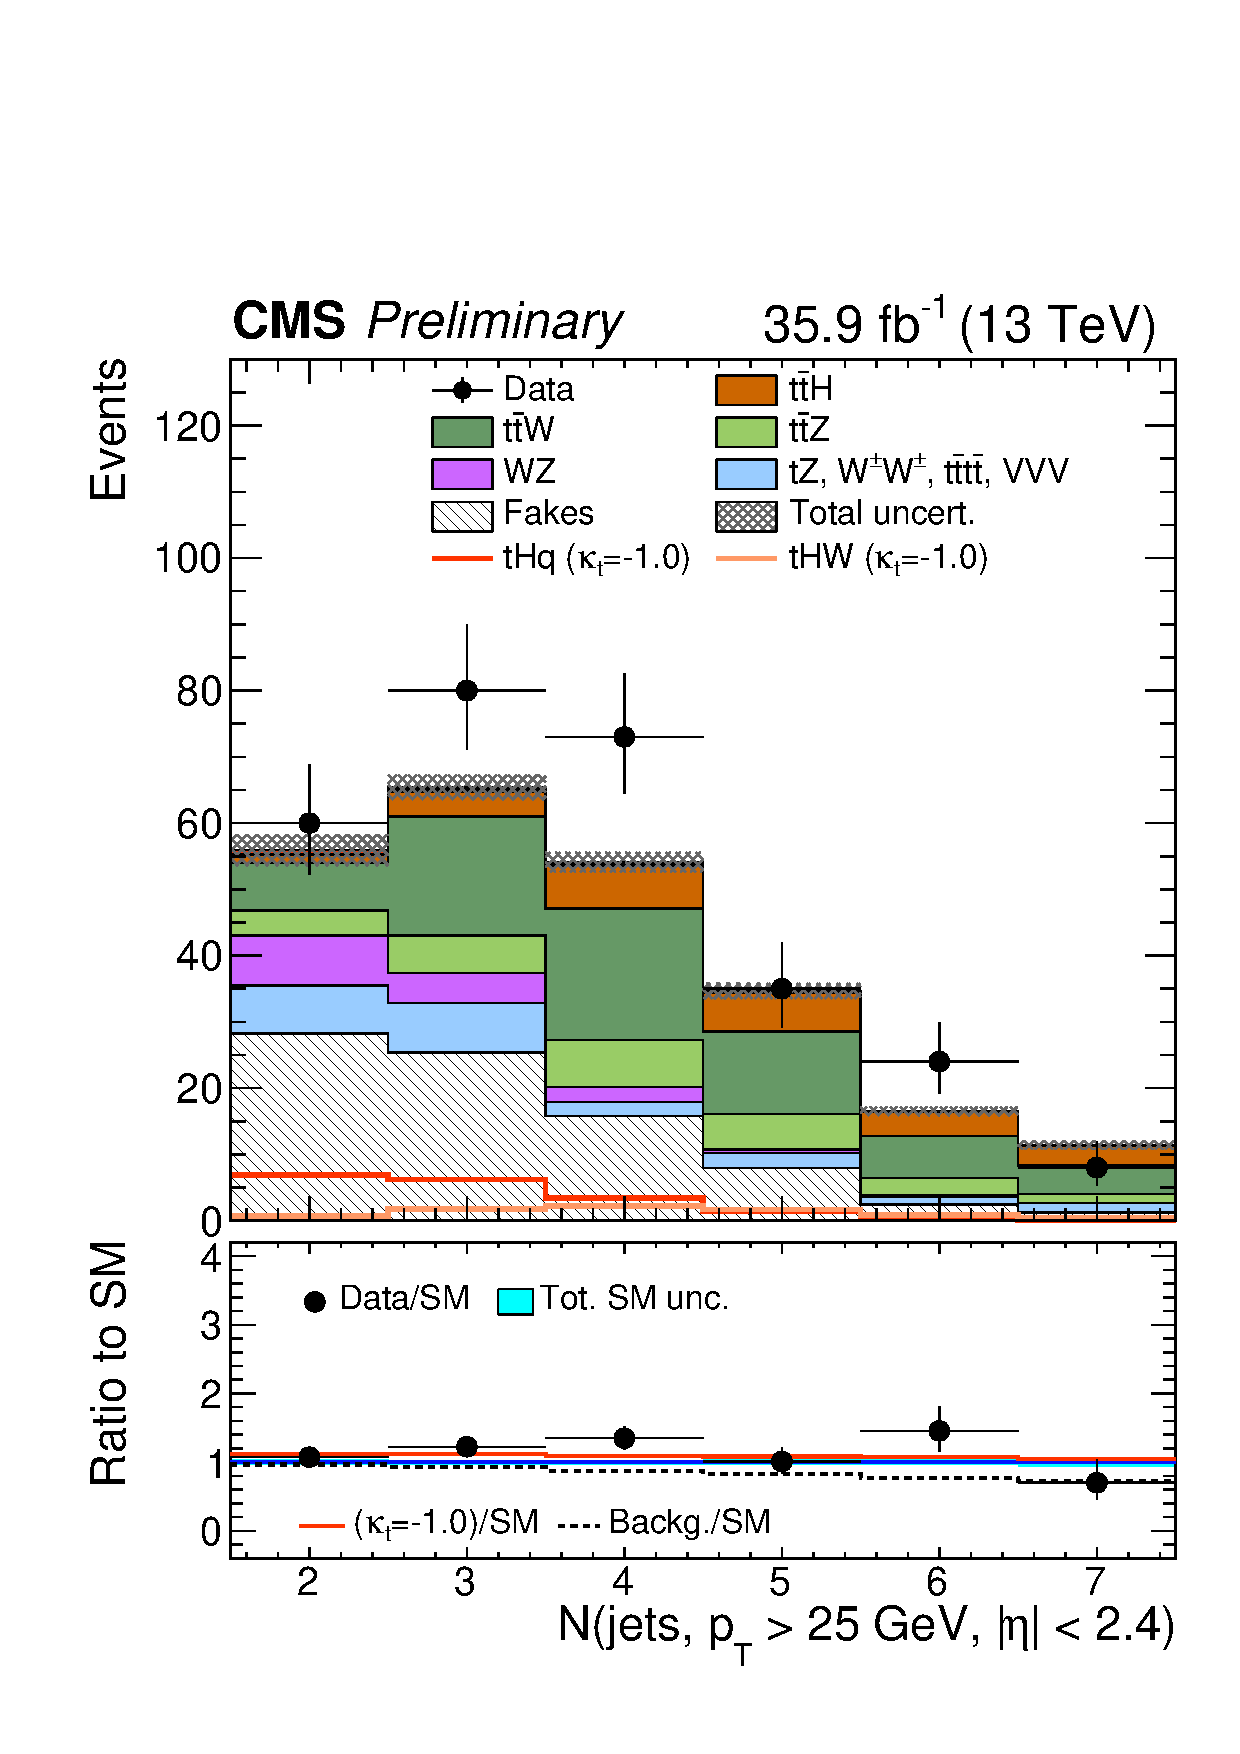
\includegraphics[width=0.32\linewidth]{Figures/polished/nJet25_mm.pdf} \\
  \caption{Distributions of discriminating variables for the event pre-selection for the same-sign \mumu\ channel, normalized to 35.9\fbinv, before fitting the signal discriminant to the observed data.
  Uncertainties are statistical and unconstrained (pre-fit) normalization systematics.
  The shape of the two \tH\ signals for $\Ct=-1.0$ is shown, normalized to their respective cross sections for $\Ct=-1.0, \CV=1.0$.\label{fig:2lss_inputs_mm}}
\end{figure}

\begin{figure}[!htb]
  \centering
    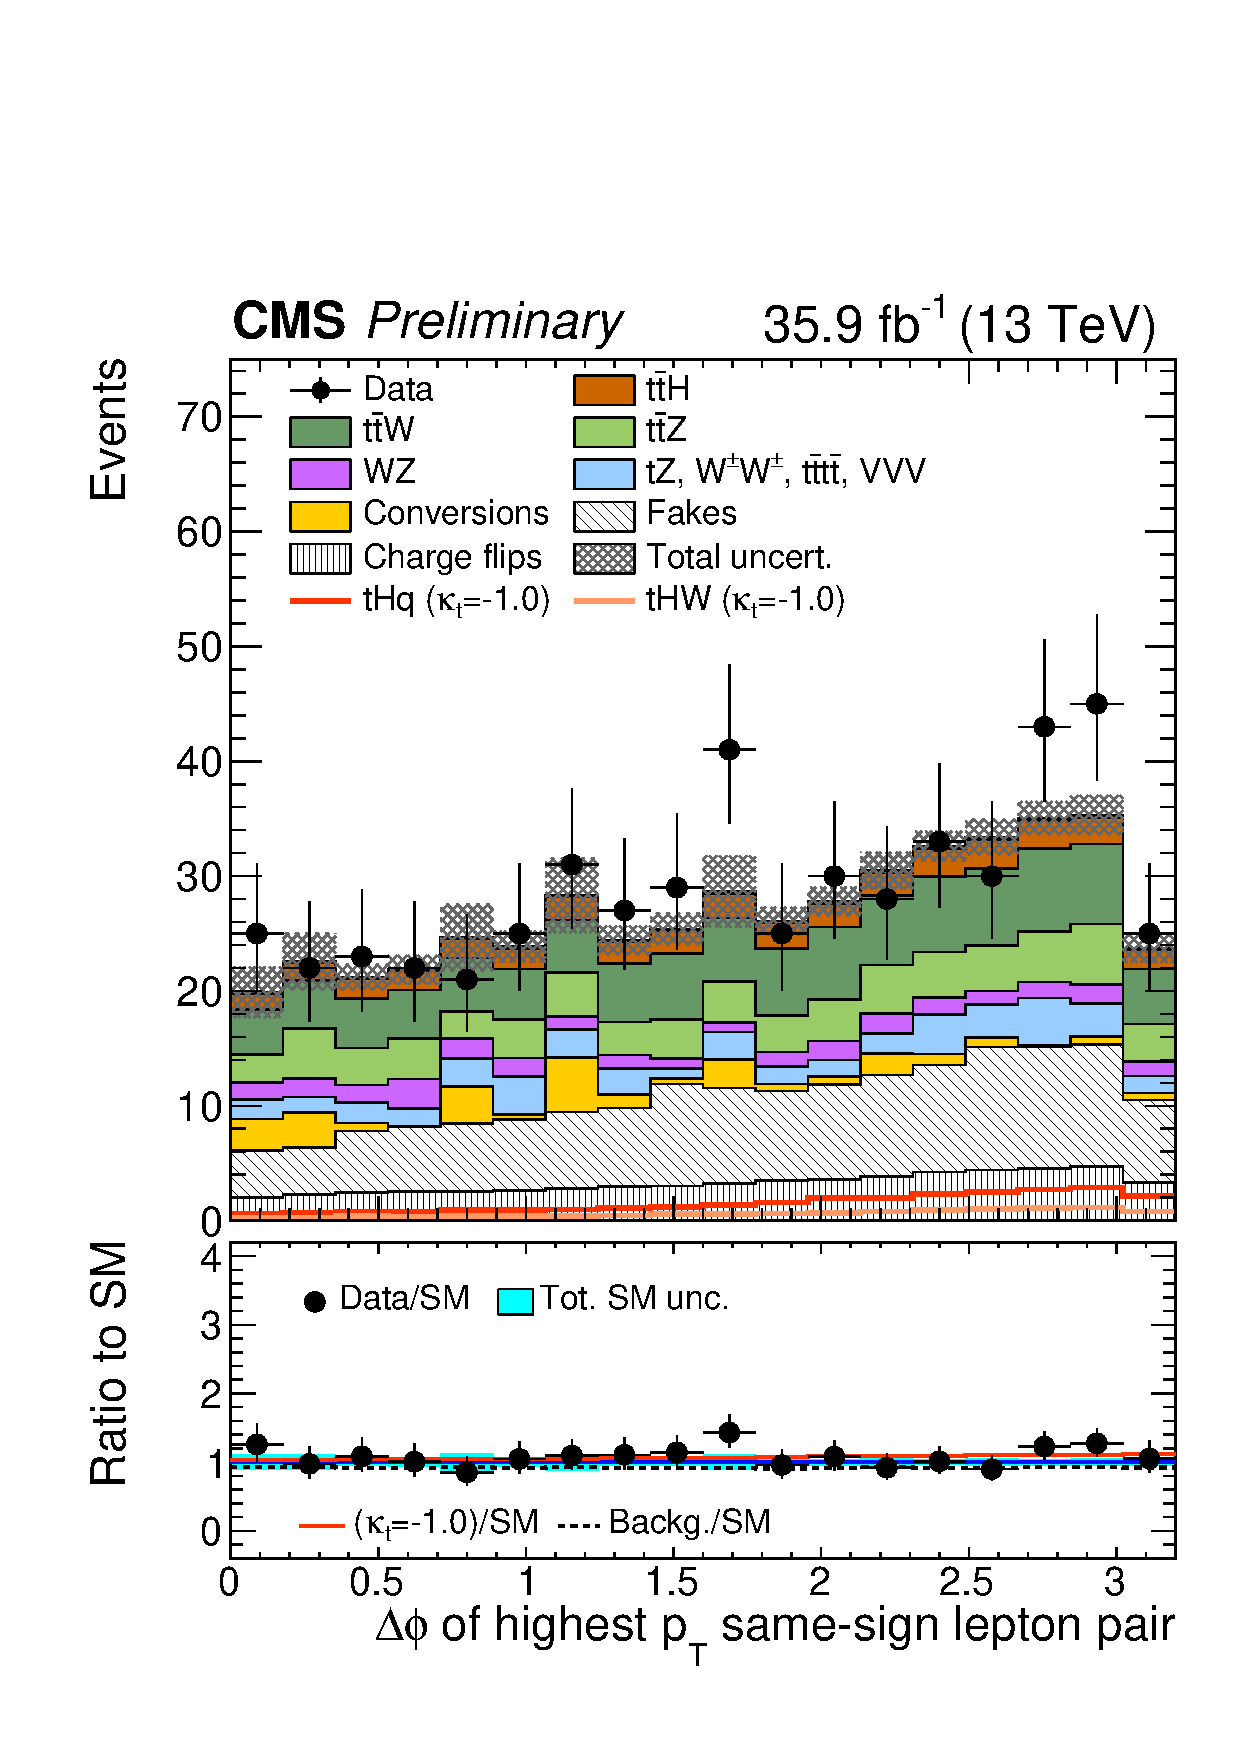
\includegraphics[width=0.32\linewidth]{Figures/polished/dPhiHighestPtSSPair_em.pdf}
    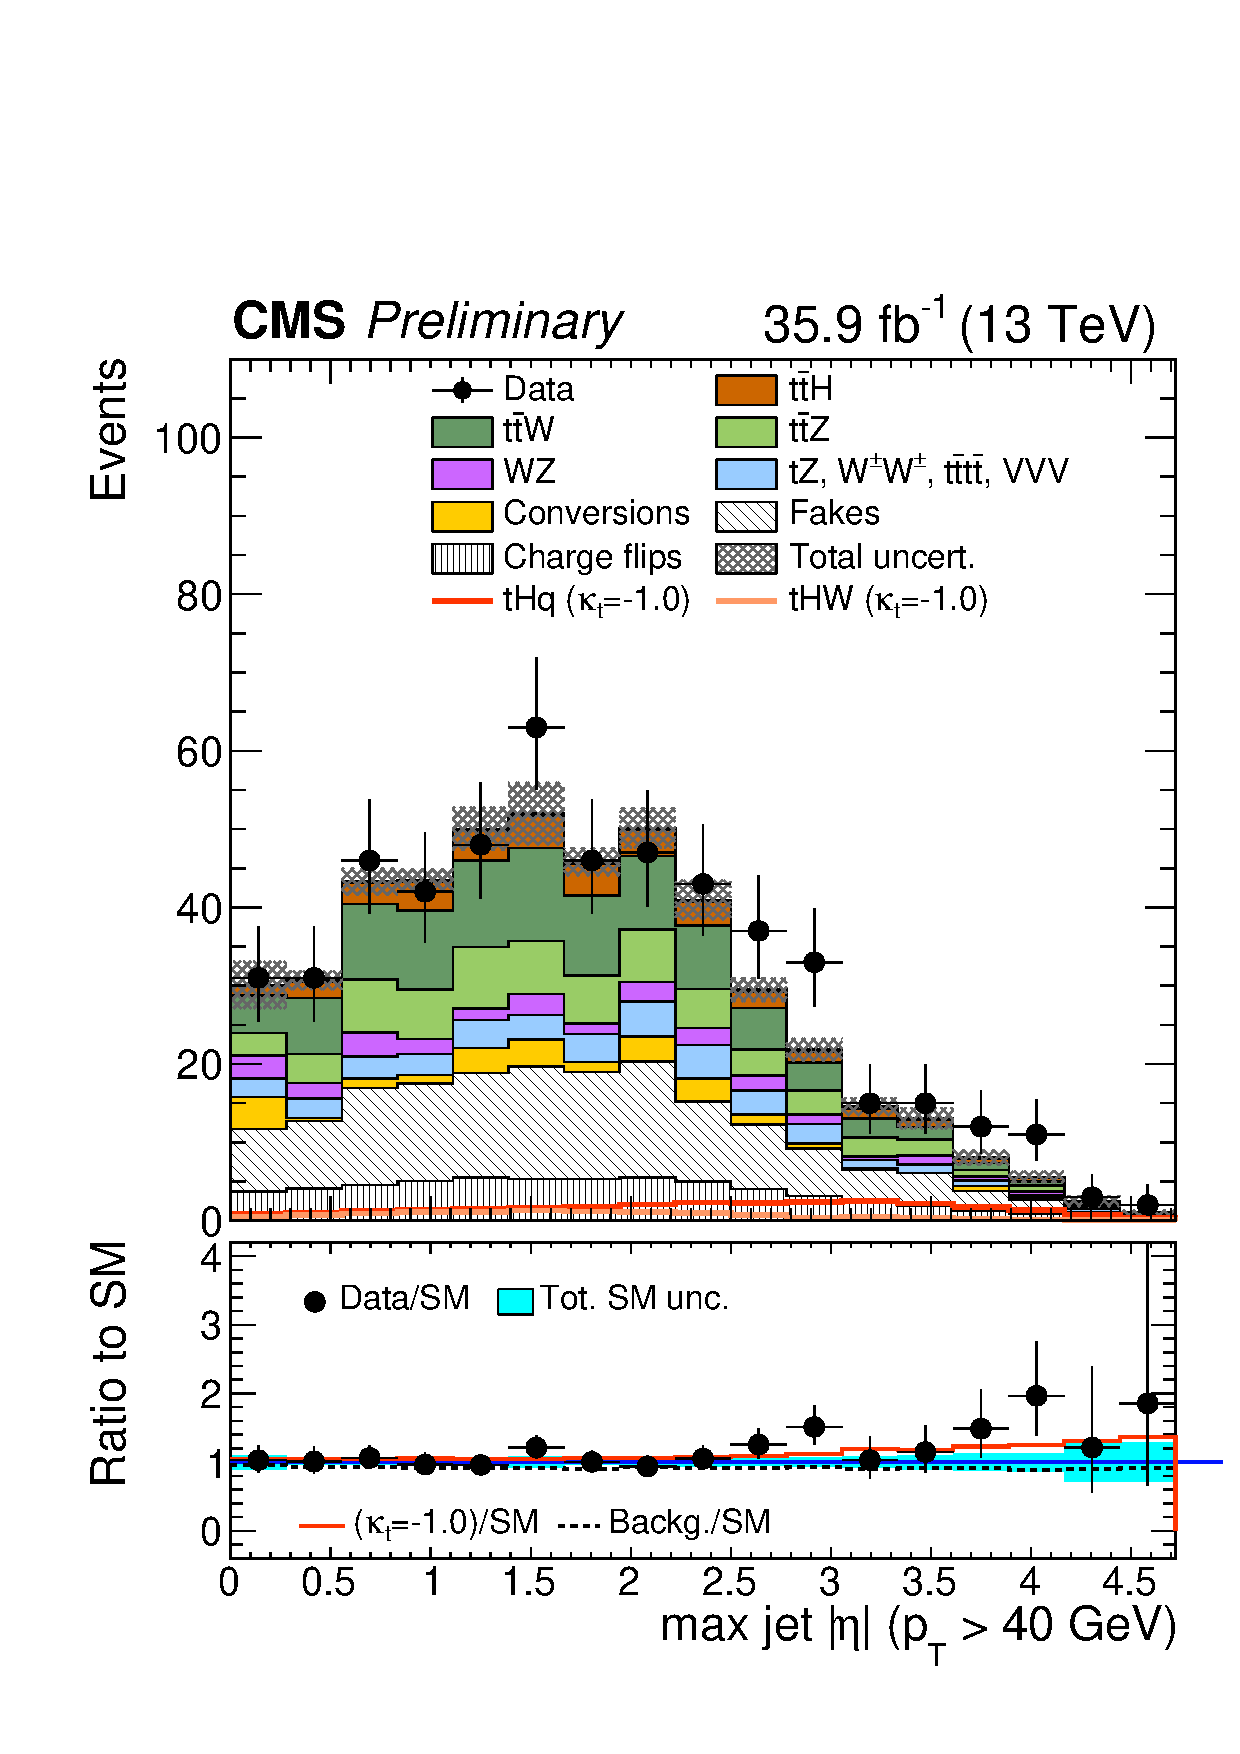
\includegraphics[width=0.32\linewidth]{Figures/polished/maxEtaJet25_40_em.pdf}
    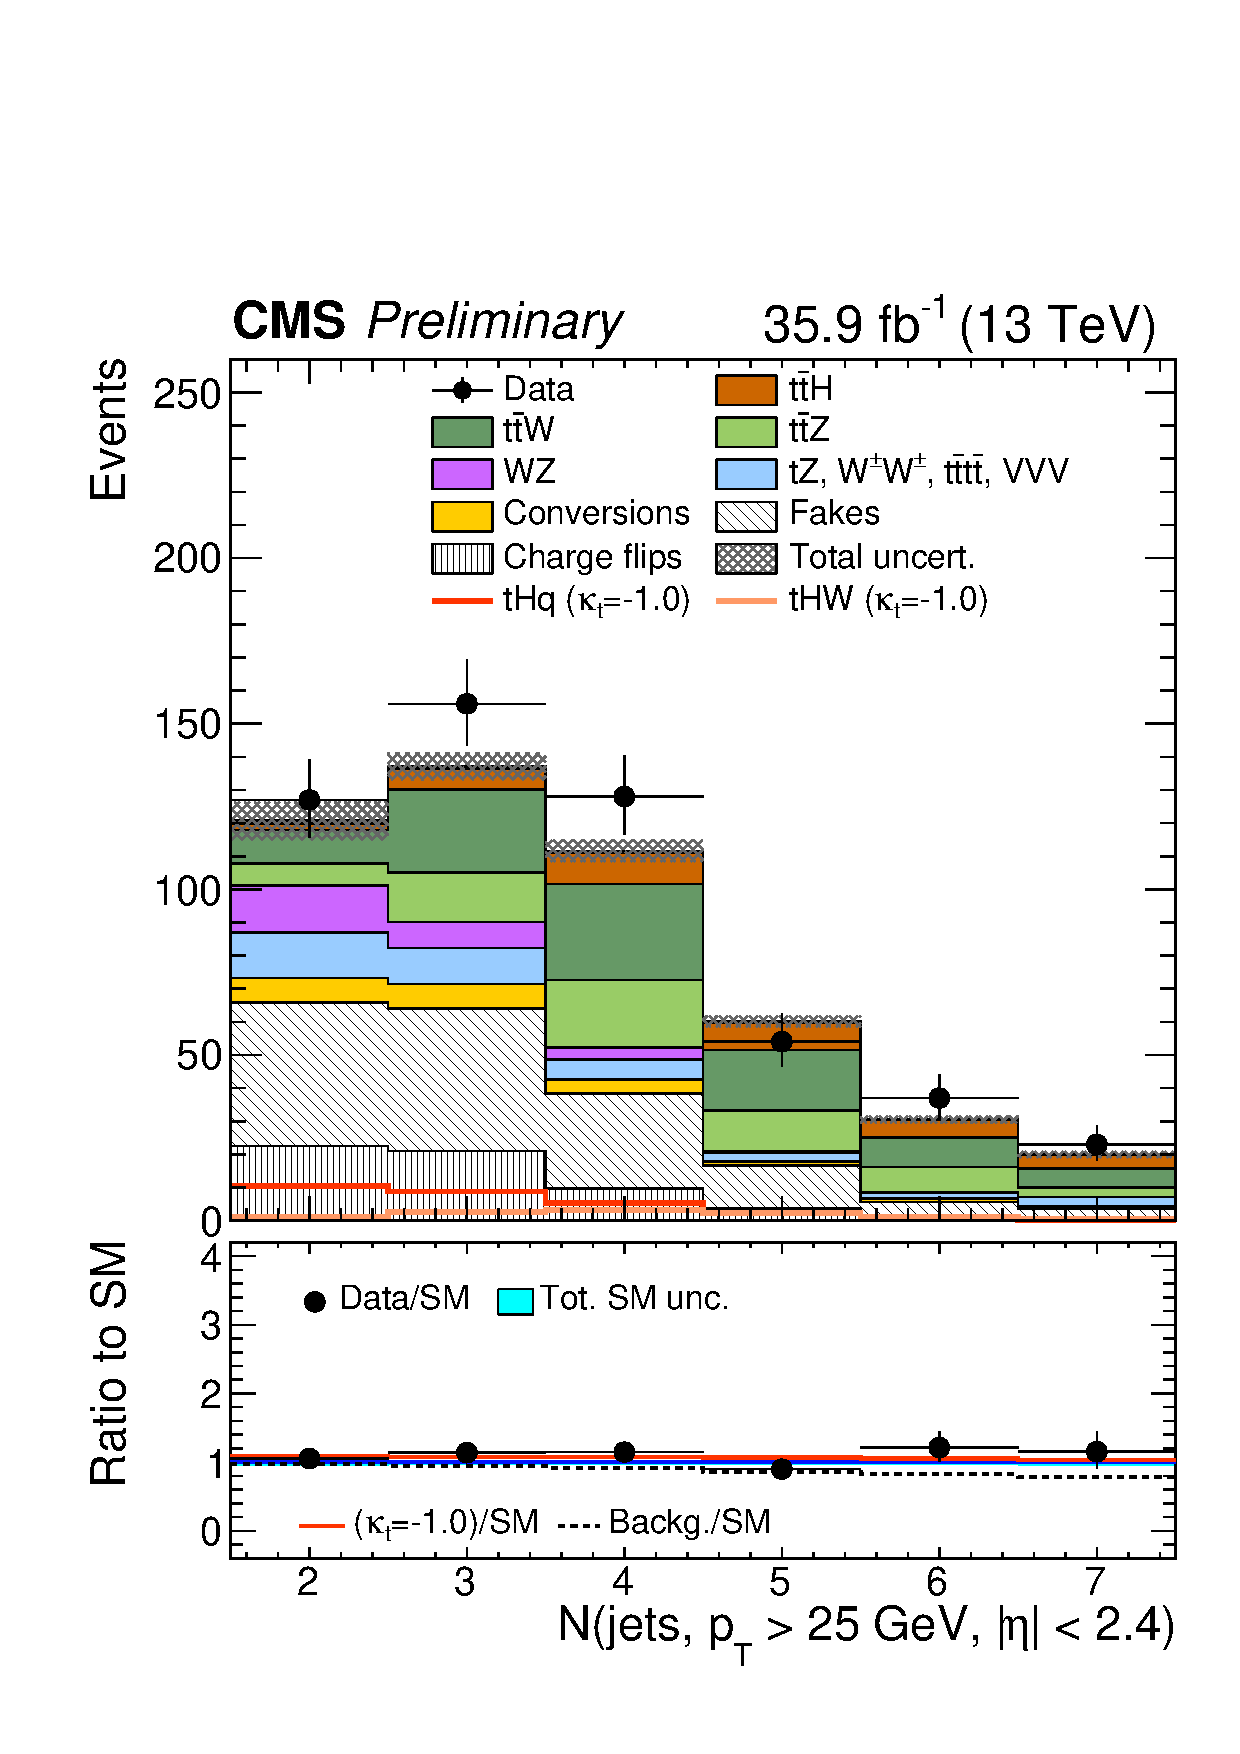
\includegraphics[width=0.32\linewidth]{Figures/polished/nJet25_em.pdf} \\
  \caption{Distributions of discriminating variables for the event
    pre-selection for the same-sign \emu\ channel, normalized to 35.9\fbinv, before fitting the signal discriminant to the observed data. Uncertainties are statistical and unconstrained (pre-fit) normalization systematics.
    The shape of the two \tH\ signals for $\Ct=-1.0$ is shown, normalized to their respective cross sections for $\Ct=-1.0, \CV=1.0$.\label{fig:2lss_inputs_em}}
\end{figure}

\begin{figure}[!htb]
  \centering
    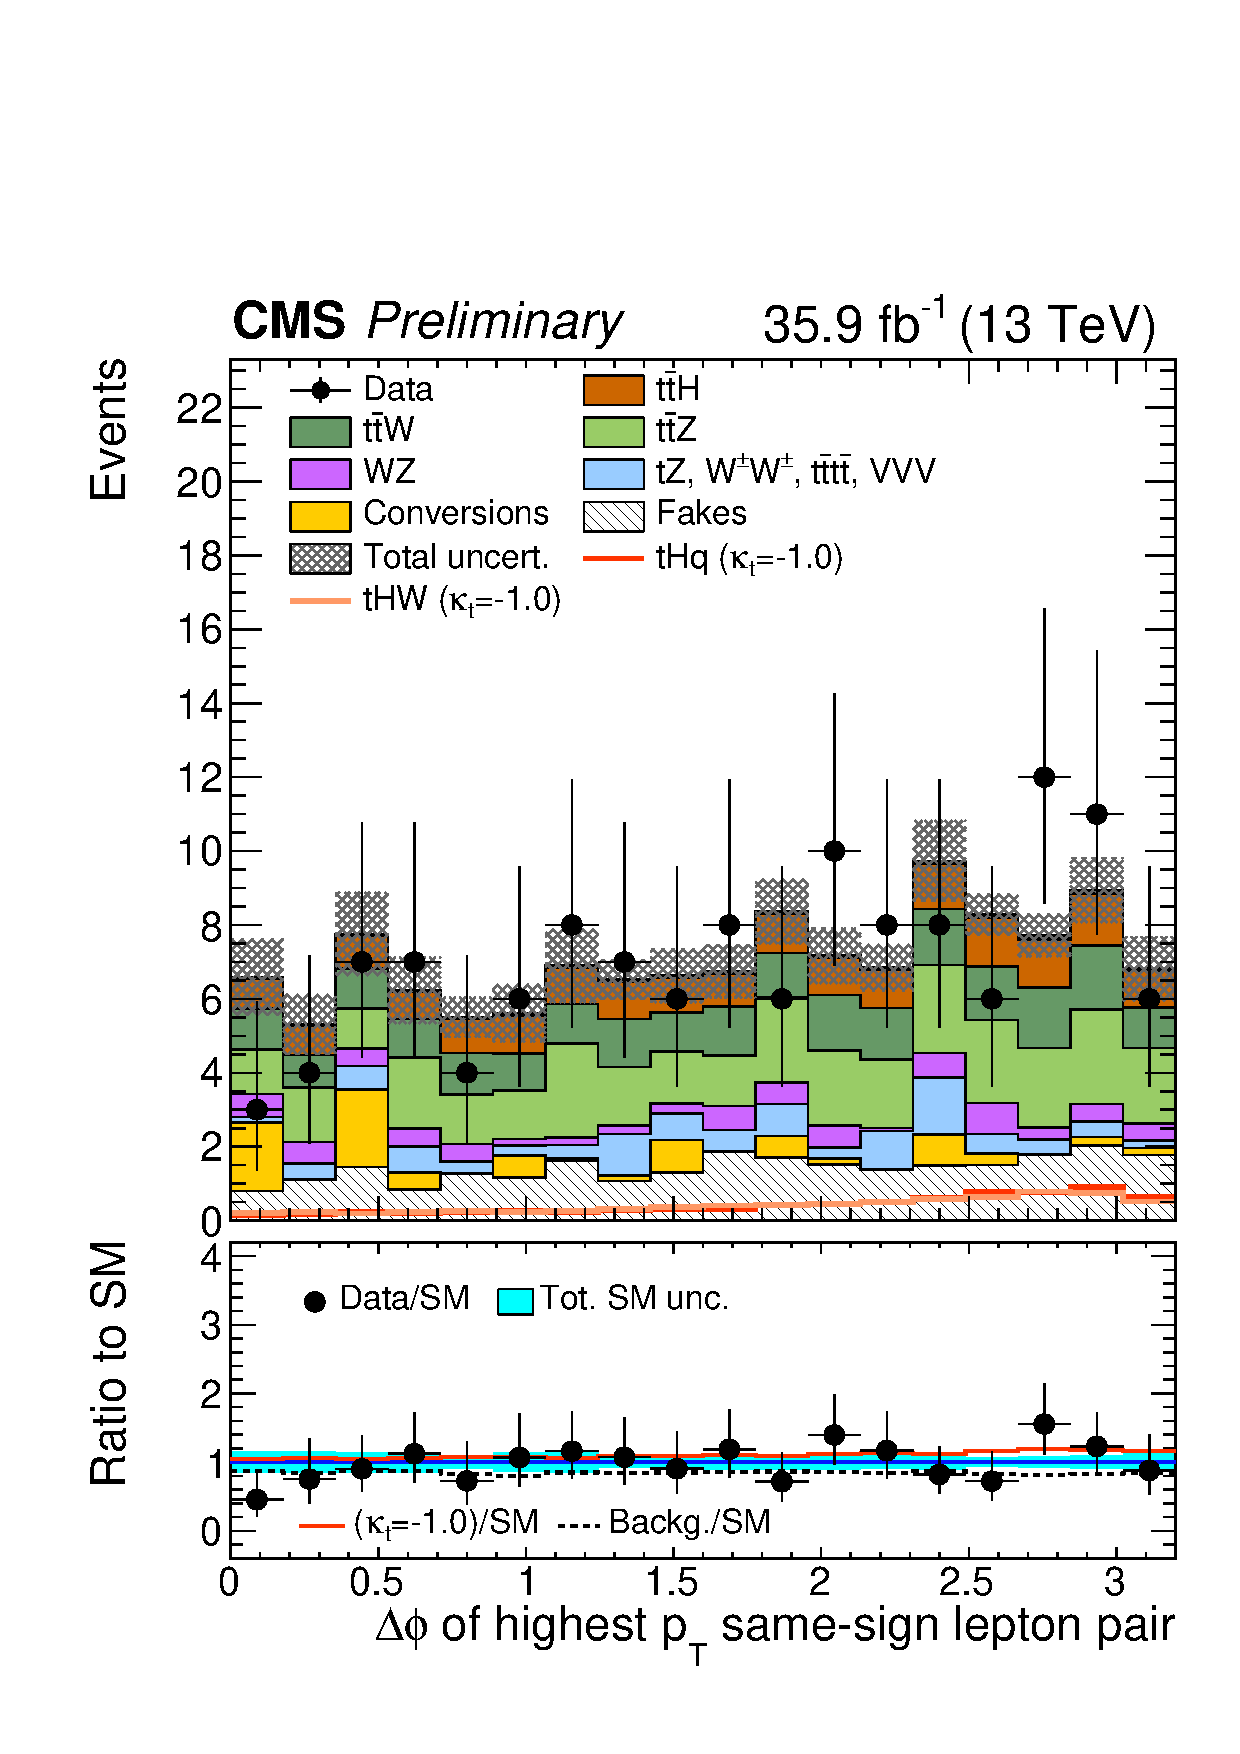
\includegraphics[width=0.32\linewidth]{Figures/polished/dPhiHighestPtSSPair_3l.pdf}
    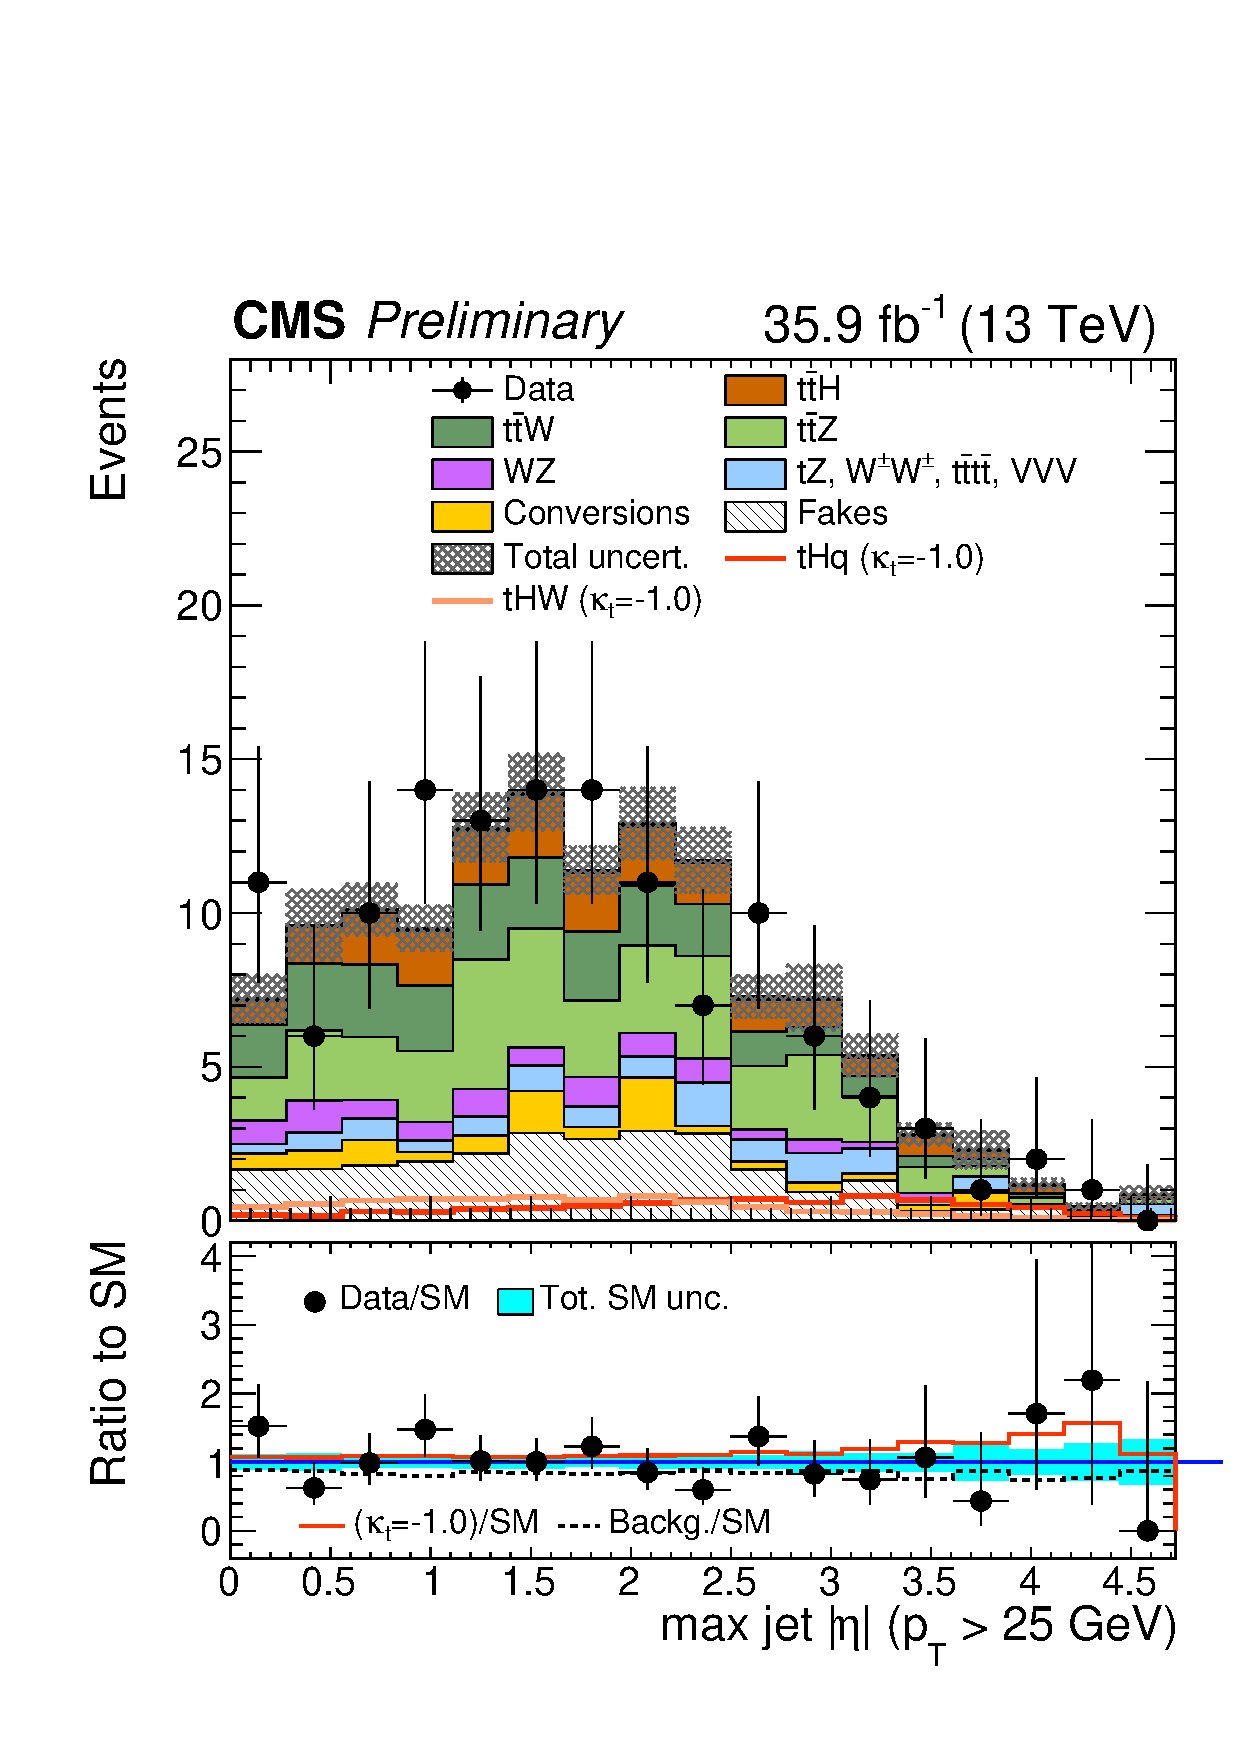
\includegraphics[width=0.32\linewidth]{Figures/polished/maxEtaJet25_40_3l.pdf}
    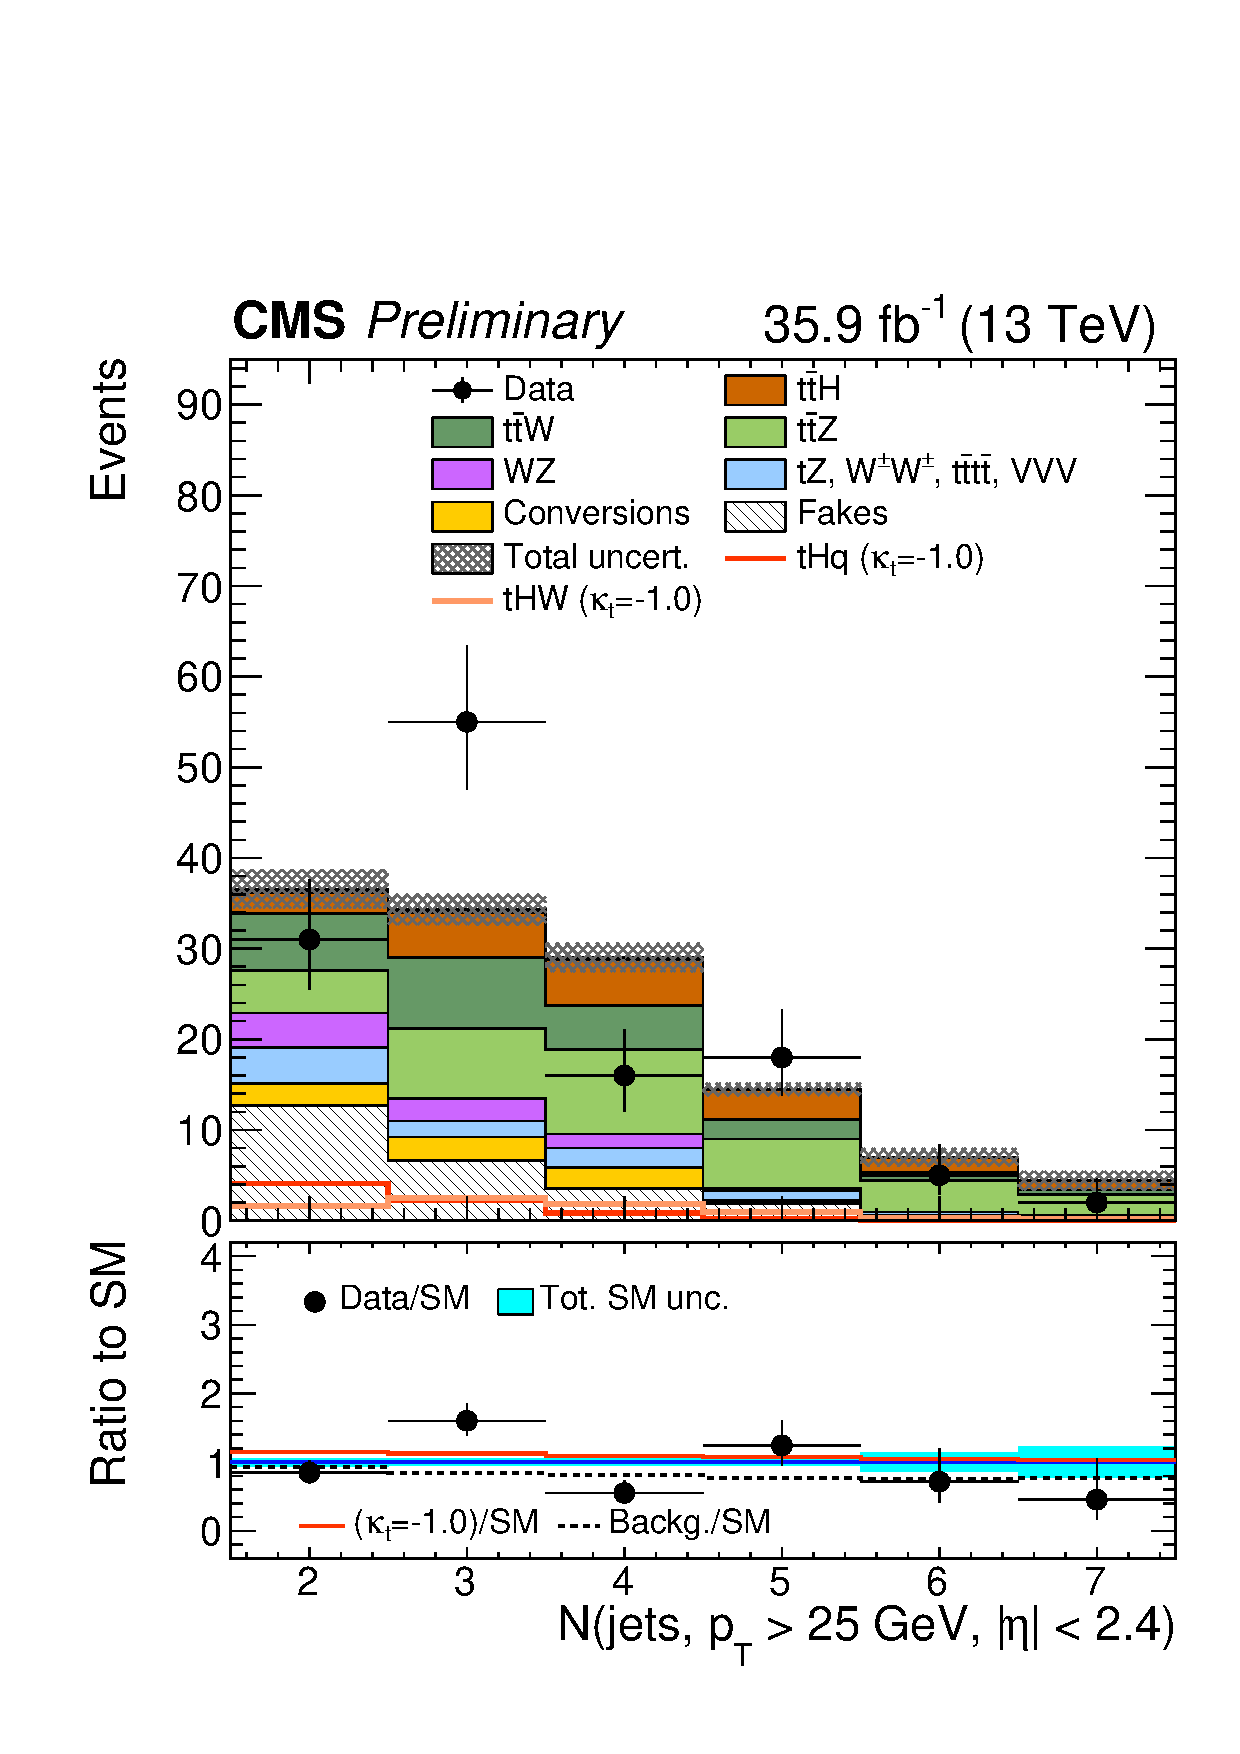
\includegraphics[width=0.32\linewidth]{Figures/polished/nJet25_3l.pdf} \\
  \caption{Distributions of discriminating variables for the event pre-selection for the three lepton channel, normalized to 35.9~\fbinv, before fitting the signal discriminant to the observed data.
  Uncertainties are statistical and unconstrained (pre-fit) normalization systematics.
  The shape of the two \tH\ signals for $\Ct=-1.0$ is shown, normalized to their respective cross sections for $\Ct=-1.0, \CV=1.0$.\label{fig:dist_likelihoodselection_PDFs_3l}}
\end{figure}
